



\section*{Введение}
Целью данное практической работы является изучение системы компьютерной верстки \LaTeX и оформление математического текста согласно стандарту ГОСТ 7.32.
\newpage

\section{МАТЕМАТИЧЕСКИЙ ТЕКСТ\label{chapter1}}
\subsection{Пример оформления математического текста}

Поскольку обе части этой формулы одновременно меняют знак при перестановке a и b, то формула справедлива при любом соотношении величин a и b,
т. е. как при a $\leq b$, так и при $a \geq b$.

На упражнениях по анализу формула Ньютона — Лейбница большей ча-
стью используется только для вычисления стоящего слева интеграла, и это
может породить несколько искаженное представление об ее использовании.
На самом деле положение вещей таково, что конкретные интегралы редко
находят через первообразную, а чаще прибегают к прямому счету на ЭВМ
с помощью хорошо разработанных численных методов. Формула Ньютона—
Лейбница занимает ключевую, связывающую интегрирование и дифферен-
цирование, позицию в самой теории математического анализа, в которой
она, в частности, получает далеко идущее развитие в виде так называемой
общей формулы Стокса

Примером того, как формула Ньютона— Лейбница используется в самом
анализе, может служить уже материал следующего пункта настоящего пара-
графа.

\subsubsection{3. Интегрирование по частям в определенном интеграле и формула Тейлора}

Утверждение 1. Если функции $u(x)$ и $v(x)$ непрерывно дифференцируемы
на отрезке с концами a и b, то справедливо соотношение \\
\begin{equation}
	\int_{a}^{b}  \,(u\cdot v)(x)dx=(u \cdot v)(x)| _a^b - \int_{a}^{b} \, (v \cdot u) (x) dx
\end{equation}

Эту формулу принято записывать в сокращенном виде
\begin{equation}
	\int_{a}^{b}  \,udv = u \cdot v | _a^b - \int_{a}^{b} \, vdu
\end{equation}

и называть формулой интегрирования по частям в определенном интеграле.

$\blacktriangleleft$ По правилу дифференцирования произведения функций имеем
\begin{center}
	$
	(u \cdot v) (x) = (u \cdot v) (x) + (u \cdot v)(x)
	$
\end{center}
По условию все функции в этом равенстве непрерывны, а значит, и инте-
грируемы на отрезке с концами a и b. Используя линейность интеграла и
формулу Ньютона— Лейбница, получаем
\begin{equation}
	(u \cdot v) (x) |^a_b = \int_{a}^{b}(u \cdot v)(x)dx+\int_{a}^{b}(u \cdot v)(x)(dx) \blacktriangleright
\end{equation}

В качестве следствия получим теперь формулу Тейлора с интегральным
остаточным членом
\\

Пусть на отрезке с концами a и x функция $t \Rightarrow  f (t)$ имеет n непрерыв-
ных производных. Используя формулу Ньютона — Лейбница,
проделаем следующую цепочку преобразований, в которых все дифференци-
рования и подстановки производятся по переменной t:

\begin{multline}
	f(x)-f(a)=\int_{a}^{x}dt = - \int_{a}^{x}f(t)(x-t)dt=\\
	= -f(t)(x-t)|^x_a + \int_{a}^{x}f(t)(x-t)dt =\\
	=f(a)(x-a)-\frac{1}{2}\int_{a}^{x}f(t)((x-t)^2)dt=\\
	=f(a)(x-a)-\frac{1}{2}f(t)(x-t)^2|^x_a+\frac{1}{2}\int^x_a f(t)(x-t)^2dt=\\
	=f(a)(x-a)+\frac{1}{2}f(a)(x-a)^2-\frac{1}{2 \cdot 3} \int^x_a f(t) (x-t)^3 dt = \dots \\
	\dots = f(a)(x-a)+\frac{1}{2}f(a)(x-a)^2 + \dots \\
	\dots + \frac{1}{2 \cdot 3 \cdot  \dots \cdot (n-1) } f^(n-1)(a)(x-a)^{n-1}+r_n-1(a;x) \\
\end{multline}
где

\begin{equation}
	r_{n-1}(a;x)=\frac{1}{(n-1)!}\int^x_a f^{(n)}(t)(x-t)^{n-1}dt	
\end{equation}
\begin{figure}[h]   
    \centering
    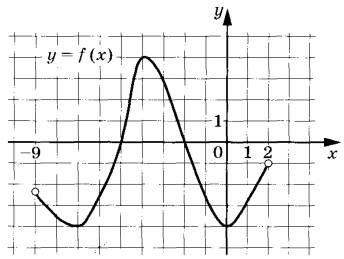
\includegraphics[width=0.7\linewidth]{img1.jpg}
    \caption{ График функции }
    \label{fig:prototype}
\end{figure}

\begin{table}[H]
	\caption{Пересечения функции с координатными осями}
	\begin{center}
		\begin{tabular}{|c|c|c|c|}
			\hline
			x & 0 & $\sqrt{3}$ & $-\sqrt{3}$ \\ \hline
			y & 1.5 & 0 & 0 \\ \hline
		\end{tabular}
		\label{tabular:tab1}
	\end{center}
\end{table}


Итак, доказано следующее

Утверждение 2. Если функция $t \Rightarrow  f (t)$ имеет на отрезке с концами a
и x непрерывные производные до порядка n включительно, то справедлива
формула Тейлора

\begin{center}
	$
	f(x)=f(a)+\frac{1}{1!}f(a)(x-a)+\dots+\frac{1}{(n-1)!}f^{(n-1)}(a)(x-a)^{n-1}+r_{n-1}(a;x)
	$
\end{center}



с остатком $r_{n-1}(a; x)$, представленным в интегральной форме.
Отметим, что функция $(x - t)^{n-1}$ не меняет знак на отрезке с концами a и
x, и поскольку функция $t\Rightarrow  f ^{(n)}(t)$ непрерывна на этом отрезке, то по первой
теореме о среднем на нем найдется такая точка $\mathfrak{Z}$ , что
\begin{multline}
	r_{n-1}(a;x)=\frac{1}{(n-1)!} f^{(n)}(t)(x-t)^{n-1}dt = \frac{1}{(n-1)!} f^(n)(\mathfrak{Z}) \int^x_a (x-t)^{n-1}dt=\\
	=\frac{1}{(n-1)!} f^{(n)}(\mathfrak{Z})(-\frac{1}{n}(x-t)^n)|^x_a=\frac{1}{n!}f^{(n)}(\mathfrak{Z})(x-a)^n
	1
\end{multline}


Мы вновь получили знакомую форму Лагранжа остаточного члена форму-
лы Тейлора. (На основании задачи 2 b) из предыдущего параграфа, можно
считать, что $\mathfrak{Z}$ лежит в интервале с концами $a, x$.)

Это рассуждение можно было бы повторить, вынося из-под знака интеграла $f (n)(\mathfrak{Z})(x - \mathfrak{Z})^{n-k}$ , где $k \in [1, n]$. Значениям $k = 1$ и $k = n$ отвечают
получаемые при этом соответственно формулы Коши и Лагранжа остаточно-
го члена.

\subsubsection{4. Замена переменной в интеграле.} Одной из основных формул ин-
тегрального исчисления является формула замены переменной в опреде-
ленном интеграле. Эта формула в теории интеграла столь же важна, как в
дифференциальном исчислении формула дифференцирования композиции
функций, с которой она может быть при определенных условиях связана
посредством формулы Ньютона— Лейбница

\cite{book}

\newpage
\section*{Заключение}
Практическая работа выполнена. Были изучены основы системы компьютерной верстки \LaTeX и оформлен математический текст согласно ГОСТ 7.32. 